% Choose one to switch between slides and handout
%\documentclass[]{beamer}
\documentclass[handout]{beamer}

% Video Meta Data
\title{Smart Contracts and Decentralized Finance}
\subtitle{Lending Protocols}
\author{Prof. Dr. Fabian Schär}
\institute{University of Basel}

% Config File
% Packages
\usepackage[utf8]{inputenc}
\usepackage{hyperref}
\usepackage{gitinfo2}
\usepackage{tikz}
 \usetikzlibrary{calc}
\usepackage{amsmath}
\usepackage{mathtools}
\usepackage{bibentry}
\usepackage{xcolor}
\usepackage{colortbl} % Add colour to LaTeX tables
\usepackage{caption}
\usepackage[export]{adjustbox}
\usepackage{pgfplots} \pgfplotsset{compat = 1.17}
\usepackage{makecell}
\usepackage{fancybox}
\usepackage{ragged2e}
\usepackage{fontawesome}
\usepackage{seqsplit}
\usepackage{tabularx}
\usepackage{tcolorbox}
\usepackage{booktabs} % use instead  \hline in tables

% Color Options
\definecolor{highlight}{rgb}{0.65,0.84,0.82}
\definecolor{focus}{rgb}{0.72, 0, 0}
\definecolor{lightred}{rgb}{0.8,0.5,0.5}
\definecolor{midgray}{RGB}{190,195,200}

 %UniBas Main Colors
\definecolor{mint}{RGB}{165,215,210}
\definecolor{anthracite}{RGB}{45,55,60}
\definecolor{red}{RGB}{210,5,55}

 %UniBas Color Palette (for graphics)
\definecolor{strongmint}{RGB}{30,165,165}
\definecolor{darkmint}{RGB}{0,110,110}
\definecolor{softanthracite}{RGB}{140,145,150}
\definecolor{brightanthracite}{RGB}{190,195,200}
\definecolor{softred}{RGB}{235,130,155}

%Custom Colors
\definecolor{lightergray}{RGB}{230, 230, 230}



% Beamer Template Options
\beamertemplatenavigationsymbolsempty
\setbeamertemplate{footline}[frame number]
\setbeamercolor{structure}{fg=black}
\setbeamercolor{footline}{fg=black}
\setbeamercolor{title}{fg=black}
\setbeamercolor{frametitle}{fg=black}
\setbeamercolor{item}{fg=black}
\setbeamercolor{}{fg=black}
\setbeamercolor{bibliography item}{fg=black}
\setbeamercolor*{bibliography entry title}{fg=black}
\setbeamercolor{alerted text}{fg=focus}
\setbeamertemplate{items}[square]
\setbeamertemplate{enumerate items}[default]
\captionsetup[figure]{labelfont={color=black},font={color=black}}
\captionsetup[table]{labelfont={color=black},font={color=black}}

\setbeamertemplate{bibliography item}{\insertbiblabel}

%tcolor boxes
\newtcolorbox{samplecode}[2][]{
  colback=mint, colframe=darkmint, coltitle=white,
  fontupper = \ttfamily\scriptsize, fonttitle= \bfseries\scriptsize,
  boxrule = 0mm, arc = 0mm,
  boxsep = 1.3mm, left = 0mm, right = 0mm, top = 0.5mm, bottom = 0mm, middle=0mm,
  #1,title=#2}
  
\newtcolorbox{keytakeaway}[2][]{
  colback=softred, colframe=red, coltitle=white,
  fontupper = \scriptsize, fonttitle= \bfseries\scriptsize,
  boxrule = 0mm, arc = 0mm,
  boxsep = 1.3mm, left = 0mm, right = 0mm, top = 0.5mm, bottom = 0mm, middle=0mm,
  #1,title=#2}

\newtcolorbox{exercise}[2][]{
  colback=brightanthracite, colframe=anthracite, coltitle=white,
  fontupper = \scriptsize, fonttitle= \bfseries\scriptsize,
  boxrule = 0mm, arc = 0mm,
  boxsep = 1.3mm, left = 0mm, right = 0mm, top = 0.5mm, bottom = 0mm, middle=0mm,
  #1,title=#2}



% Link Icon Command 
\newcommand{\link}{%
    \tikz[x=1.2ex, y=1.2ex, baseline=-0.05ex]{%
        \begin{scope}[x=1ex, y=1ex]
            \clip (-0.1,-0.1)
                --++ (-0, 1.2)
                --++ (0.6, 0)
                --++ (0, -0.6)
                --++ (0.6, 0)
                --++ (0, -1);
            \path[draw,
                line width = 0.5,
                rounded corners=0.5]
                (0,0) rectangle (1,1);
        \end{scope}
        \path[draw, line width = 0.5] (0.5, 0.5)
            -- (1, 1);
        \path[draw, line width = 0.5] (0.6, 1)
            -- (1, 1) -- (1, 0.6);
        }
    }

% Other commands
\newcommand\tab[1][0.5cm]{\hspace*{#1}} % for code boxes


% Read Git Data from Github Actions Workflow
% Defaults to gitinfo2 for local builds
\IfFileExists{gitInfo.txt}
	{\input{gitInfo.txt}}
	{
		\newcommand{\gitRelease}{(Local Release)}
		\newcommand{\gitSHA}{\gitHash}
		\newcommand{\gitDate}{\gitAuthorIsoDate}
	}

% Custom Titlepage
\defbeamertemplate*{title page}{customized}[1][]
{
  \vspace{-0cm}\hfill\includegraphics[width=2.5cm]{../config/logo_cif}
  \includegraphics[width=1.9cm]{../config/seal_wwz}
  \\ \vspace{2em}
  \usebeamerfont{title}\textbf{\inserttitle}\par
  \usebeamerfont{title}\usebeamercolor[fg]{title}\insertsubtitle\par  \vspace{1.5em}
  \small\usebeamerfont{author}\insertauthor\par
  \usebeamerfont{author}\insertinstitute\par \vspace{2em}
  \usebeamercolor[fg]{titlegraphic}\inserttitlegraphic
    \tiny \noindent \texttt{Release Ver.: \gitRelease}\\ 
    \texttt{Version Hash: \gitSHA}\\
    \texttt{Version Date: \gitDate}\\ \vspace{1em}
    
    
    \iffalse
  \link \href{https://github.com/cifunibas/Bitcoin-Blockchain-Cryptoassets/blob/main/slides/intro.pdf}
  {Get most recent version}\\
  \link \href{https://github.com/cifunibas/Bitcoin-Blockchain-Cryptoassets/blob/main/slides/intro.pdf}
  {Watch video lecture}\\ 
  
  \fi
  
  \vspace{1em}
  License: \texttt{Creative Commons Attribution-NonCommercial-ShareAlike 4.0 International}\\\vspace{2em}
  \includegraphics[width = 1.2cm]{../config/license}
}


% tikzlibraries
\usetikzlibrary{decorations.pathreplacing}
\usetikzlibrary{decorations.markings}
\usetikzlibrary{positioning}
\usetikzlibrary{calc}
\captionsetup{font=footnotesize}

%%%%%%%%%%%%%%%%%%%%%%%%%%%%%%%%%%%%%%%%%%%%%%
%%%%%%%%%%%%%%%%%%%%%%%%%%%%%%%%%%%%%%%%%%%%%%
\begin{document}

\thispagestyle{empty}
\begin{frame}[noframenumbering]
	\titlepage
\end{frame}

%%%
\begin{frame}{Protocol Layer}

\begin{figure}[t]
	\centering
	\resizebox{0.9\textwidth}{!}{
	\begin{tikzpicture}[scale=1.0, every node/.style={scale=1.0}]
		\input{../assets/figures/defi_stack_protocol_layer_lending}
	\end{tikzpicture}}
	\caption{DeFi Stack \cite{FS:21}}
\end{figure}
	
\end{frame}
%%%	


%%%
\begin{frame}{Introduction}
\textbf{Borrowing} and \textbf{lending} are basic needs in any financial system. \\

\vspace{1em}

\uncover<2-> {
Loans exist in various forms, but they usually require at least one of the two following properties:
\vspace{0.5em}
\begin{enumerate}
  \item \textbf{Collateral:} Loan is secured with specific assets.
  \item \textbf{Verifiable Identities:} Option to take legal action.
\end{enumerate} 
}

\vspace{1em}
\uncover<3->{
	In DeFi, verifiable identities are the exception. Loans are therefore mostly (over-)collateralized.
}

\end{frame}
%%%	


%%%
\begin{frame}{Some Terminology Around Lending in DeFi}

\vspace{1em}

\textbf{Position}: Entirety of an address' collateral $c$ and debt $d$ with a given lending protocol.
			
\vspace{1.0em}
			
\uncover<2-> {
\textbf{Loan-to-Value} (\textit{$LTV_i$}): $LTV_i \in [0,1]$ is a protocol parameter that determines the fraction of asset $i$ that counts towards the liquidity provider's borrowing capacity.
}

\vspace{1.0em}

\uncover<3->{ 
\textbf{Borrowing Capacity} ($BC$): $BC \geq 0$ is the sum of $LTV$-adjusted values across all collateral types in a given position. It determines the maximum value that can be borrowed against the position's collateral.
%
\begin{equation*}
	BC = \sum c_i\, LTV_i 
	\label{eq:BC} 
\end{equation*}
}

\end{frame}
%%%	


%%%
\begin{frame}{Some Terminology Around Lending in DeFi}

\vspace{1em}

\textbf{Relative Liquidation Threshold} ($rLT_i$): $rLT_i \in [0,1]$ is a protocol parameter that determines the fraction of asset $i$ that counts towards the liquidity provider's liquidation threshold. \vspace{1em}

\uncover<2->{
\textbf{Absolute Liquidation Threshold} ($aLT$): $aLT \geq 0$ is the sum of $rLT$-adjusted values across all collateral types in a given position. It determines the maximum debt of a position may accumulate against its collateral, before being open for liquidation.
%
\begin{equation*}
	aLT = \sum c_i\, rLT_i 
	\label{eq:LT} 
\end{equation*}
}

\uncover<3->{
\begin{keytakeaway}{Relationship Between $BC$ and $aLT$ / $LTV_i$ and $rLT_i$}
	Note, that $BC$ and $aLT$ are closely related. The former determines the maximum debt that can be borrowed with a specific collateral mix, while the latter determines the debt value threshold at which the position can be liquidated. The difference between $BC$ and $aLT$ is a safety cushion for borrowers. Similarly, $LTV_i$ and $rLT_i$ are the corresponding collateral factors for a given collateral type $i$.
\end{keytakeaway}
}

\end{frame}
%%%

%%%
\begin{frame}{Some Terminology Around Lending in DeFi}
\textbf{Health Factor} (HF): HF is the ratio between a position's $aLT$ and the sum of any outstanding debt. It can only be computed for positions with $\sum d_i > 0$; otherwise irrelevant.

\begin{equation*}
	  HF = \frac{\sum c_i \, rLT_i}{\sum d_i} =  \frac{aLT}{\sum d_i} 
	  \label{eq:HF} 
\end{equation*}

\vspace{1.0em}
\begin{keytakeaway}{Health Factor and Liquidations}
\begin{itemize}
	\item A position with $HF \geq 1$ is considered \textbf{healthy}.
	\item A position with $HF < 1$ is considered \textbf{unhealthy} and can be liquidated by anyone.
\end{itemize}
\end{keytakeaway}



\end{frame}

%%%
\begin{frame}{Two Approaches to Collateralized Loans}
	\vspace{1em}
	There are two collateralized lending protocol archetypes in DeFi: \textbf{Collateralized Debt Positions} (CDP) and \textbf{Collateralized Debt Markets} (CDM).\\ \vspace{1em}

	\begin{itemize}
		\item \textbf{CDPs} allow borrowers to lock collateral and thereby mint new liquid assets on demand.
		\item \textbf{CDMs} are used to match the borrowers' and lenders' demands in an aggregated pool. There are no new assets created.
	\end{itemize}
	
\end{frame}


%%%
\begin{frame}{Collateralized Debt Position (CDP)}

\vspace{-1em}

\begin{figure}[t]
	\centering
	\begin{tikzpicture}[scale=1.0, every node/.style={scale=1.0}]
		
% Figures

\node (borrower) at (-8,0) {\includegraphics[height = 1.7cm]{../assets/images/agents/handing_right}};
\node [below of = borrower, yshift = -0.4cm] {\textbf{Alice}};

\node (protocol) at (0,0) {\includegraphics[height = 1.7cm]{../assets/images/smart_contract}};
\node [below of = protocol, yshift = -0.4cm] {\textbf{CDP}};

% Arrows with text

\footnotesize

\uncover<2->{
\draw[->, black]	([yshift=0.2cm]borrower.east) -- ([yshift=0.2cm]protocol.west) node[midway, fill=white, text = darkmint, align = center] {\textbf{Asset $X$}};
}

\uncover<3->{
\draw[<-, black]	([yshift=-0.2cm]borrower.east) -- ([yshift=-0.2cm]protocol.west) node[midway, fill=white, text = darkmint, align = center] {\textbf{Loan in newly minted $Y$}};
}

	\end{tikzpicture}
\end{figure}


\small

\begin{enumerate}
	\item<2-> {Alice provides assets (collateral) of type $X$ to CDP.}
	\item<3-> {Alice may call function in CDP to mint and borrow $Y$-tokens. Her $X$-tokens on the CDP are used as collateral.}
\end{enumerate}

\uncover<4->{
Alice pays interest (sometimes referred to as stability fee) for the outstanding debt in $Y$. She still participates in any price movements of $X$, while getting a liquid asset $Y$ for consumption or further investments (leverage).
}
	
\end{frame}
%%%	


%%%
\begin{frame}{Collateralized Debt Markets (CDM)}


\vspace{-1em}

\begin{figure}[t]
	\centering
	\begin{tikzpicture}[scale=1.0, every node/.style={scale=1.0}]
		
% Figures

\node (borrower) at (-4.6,0) {\includegraphics[height = 1.7cm]{../assets/images/agents/handing_right}};
\node [below of = borrower, yshift = -0.4cm] {\textbf{Alice}};

\node (protocol) at (0,0) {\includegraphics[height = 1.7cm]{../assets/images/smart_contract}};
\node [below of = protocol, yshift = -0.4cm] {\textbf{CDM}};

\node (lender) at (4.6,0) {\includegraphics[height = 1.7cm]{../assets/images/agents/handing_left}};
\node [below of = lender, yshift = -0.4cm] {\textbf{Bob}};


% Arrows with text

\footnotesize

\uncover<2->{
\draw[->, black]	([yshift=0.6cm]borrower.east) -- ([yshift=0.6cm]protocol.west) node[midway, fill=white, text width = 1.6cm, text = darkmint, align = center] {\textbf{Asset $X$}};

\draw[<-, black]	([yshift=0.2cm]borrower.east) -- ([yshift=0.2cm]protocol.west) node[midway, fill=white, text width = 1.6cm, text = darkmint, align = center] {\textbf{$IBT_X$}};
}

\uncover<4->{
\draw[<-, black]	([yshift=-0.4cm]borrower.east) -- ([yshift=-0.4cm]protocol.west) node[midway, fill=white, text width = 1.6cm, text = darkmint, align = center] {\textbf{Loan in $Y$}};

%\draw[->, black]	([yshift=-0.7cm]borrower.east) -- ([yshift=-0.7cm]protocol.west) node[midway, fill=white, text width = 1.6cm, text = darkmint, align = center] {\textbf{Interest $Y$}};
}

\uncover<3->{
\draw[->, black]	([yshift=0.25cm]lender.west) -- ([yshift=0.25cm]protocol.east) node[midway, fill=white, text width = 1.2cm, text = darkmint, align = center] {\textbf{Asset $Y$}};

\draw[<-, black]	([yshift=-0.15cm]lender.west) -- ([yshift=-0.15cm]protocol.east) node[midway, fill=white, text width = 1.2cm, text = darkmint, align = center] {\textbf{$IBT_Y$}};
}

	\end{tikzpicture}
\end{figure}

\vspace{-1em}

\small

\begin{enumerate}
	\item<2-> {Alice provides assets (collateral) of type $X$ to CDM and receives interest bearing tokens ($IBT_X$) in return.}
	\item<3-> {Bob provides assets (collateral) of type $Y$ to CDM and receives interest bearing tokens ($IBT_Y$) in return.}
	\item<4-> {Alice borrows tokens of type $Y$. Her $X$-tokens on the CDM are used as collateral.}
\end{enumerate}

\uncover<5->{
Alice pays interest for the outstanding debt in $Y$ and receives interest for her $X$-collateral. Bob receives interest for the provision of $Y$. Interest rates are determined as a function of the pool utilization for the respective asset. 
}
	
\end{frame}
%%%	


%%%
\begin{frame}{Interest Bearing Tokens}

In CDMs, participants receive \emph{interest bearing tokens} for the assets provided. The tokens...
\vspace{0.5em}
\begin{itemize}
  \item ...represent \textbf{transferable claims} to the collateral,
  \item ...\textbf{account for interest} earned
  \item ...are \textbf{burnt to redeem and withdraw} the assets incl. accrued interest.
\end{itemize}

\uncover<2-> {
\vspace{1.0em}
\begin{keytakeaway}{Interest Earned is Not Risk Free}
	Protocol malfunctions or tail events that block necessary liquidations may leave lenders with interest bearing tokens, that cannot be (fully) redeemed. These situations may be temporary or permanent.
\end{keytakeaway}
}

\end{frame}
%%%	


%%%
\begin{frame}{Comparison of Two Interest Bearing Token Models}

\footnotesize
\begin{table}
  \center
  \begin{tabularx}{\textwidth}{rXX}
    \toprule
    ~	& \textbf{Aave V2} \emph{aToken} & \textbf{Compound} \emph{cToken}	\\
    \midrule
    \textbf{Naming} & a\textit{Reserve} (e.g., aDai) & c\textit{Reserve} (e.g., cDai) \vspace{0.5em}\\
    \textbf{Redemption} & 1:1 & $cToken \cdot XRate_{reserve}$ \vspace{0.5em}\\
    \textbf{Interest Logic} & Base rate + two slopes split by optimal utilization. & Base rate + one slope \textbf{or} two slopes split by optimal utilization. \vspace{0.5em}\\
    %\textbf{Security Reserve} & By reserve asset. Held by treasury as aToken. & By reserve asset. Value stored in each contract. \vspace{0.5em}\\
    \textbf{Interest Calculation} & Per second. With every tx affecting debt or liquidity balances. & Per block. With every tx affecting debt or liquidity balances. \vspace{0.5em}\\
    \textbf{Interest Model} & Stable and variable rates. & Variable rates only. \vspace{0.5em}\\
    \textbf{Liquidator} & Can choose between reserve asset and aToken. & Gets cToken.\\
    \bottomrule
  \end{tabularx}
  \caption{Comparison aToken and cToken \cite{AaveV2,Compound}}
\end{table}

\end{frame}
%%%	


%%%
\begin{frame}{CDM: Interest as a Function of Utilization }

Most CDM protocols have a variable borrower interest rate $r_b$. It is usually a \textbf{function of the utilization ratio} $u_t$, i.e., the ratio between borrowed liquidity $D_t$ and provided liquidity $L_t$.

\vspace{1.5em}

\uncover<2-> {
\begin{minipage}{0.6\textwidth}
	\begin{figure}[t]
		\centering
		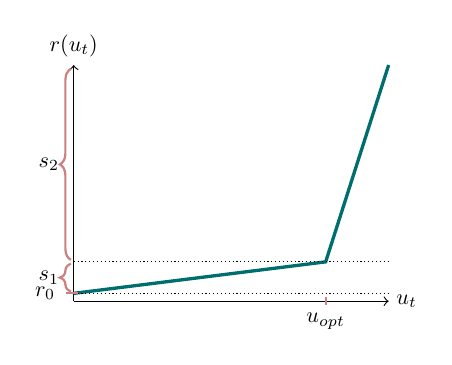
\begin{tikzpicture}[scale=0.5, every node/.style={scale=0.8}]
			
% Axis

\draw[->] (0,0) -- (0,6) node [above ]{$r(u_t)$};
\draw[->] (0,0) -- (8,0) node [right] {$u_t$};


% Slopes and lines

\draw [darkmint, very thick](0,0.2) -- (6.4,1) -- (8,6);

\draw [densely dotted, thin] (0,1) -- (8,1);
\draw [densely dotted, thin] (0,0.2) -- (8,0.2);

% Labels and Braces

\draw [thick, lightred] (6.4,0.1) -- (6.4,-0.1) node [below, align = center, text = black] {$u_{opt}$};

\draw [thick, lightred] (-0.2,0.2) -- (0.1,0.2) node [xshift = -6.5pt, left, align = right, text = black] {$r_0$};

%\draw [decorate,decoration={brace,amplitude=2pt},xshift=-2pt,yshift=0pt](0,0) -- (0.0,0.12) node [black,midway,xshift=-0.3cm] {$r_0$};

\draw [decorate,decoration={brace,amplitude=4pt},xshift=-2pt,yshift=0pt, lightred, thick](0,0.25) -- (0.0,0.95) node [black,midway,xshift=-0.35cm] {$s_1$};

\draw [decorate,decoration={brace,amplitude=4pt},xshift=-2pt,yshift=0pt, lightred, thick](0,1.05) -- (0,5.9) node [black,midway,xshift=-0.35cm] {$s_2$};
		\end{tikzpicture}
		\caption{Dual Interest Slope}
	\end{figure}
\end{minipage}
\begin{minipage}{0.38\textwidth}
	\vspace{-1em}
	\begin{equation*}
		u_t = \dfrac{D_t}{L_t}
	\end{equation*}
	
	\vspace{0.5 em}
	Most interest functions are defined by logical cases, that allow for varying slopes. 
	
\end{minipage}	
}

\end{frame}
%%%	


%%%
\begin{frame}{CDM: Borrower's Interest and Lender's Yield }

In a CDM with two distinct slope intervals, the borrower's interest rate $r_b$ is a two-case function of $u_t$, with the protocol parameters $r_{min}, r_{opt}, r_{max}$ and $u_{opt}$:

\begin{equation*}
	r_b = 
		\begin{cases}
		r_{min} + \dfrac{u_t}{u_{opt}}(r_{opt}-r_{min}), & \text{if } u_t \leq u_{opt} \vspace{1em}\\
		r_{opt} + \dfrac{u_t-u_{opt}}{1-u_{opt}}(r_{max}-r_{opt}), & \text{if } u_t > u_{opt}
		\end{cases}
\end{equation*}

\vspace{1em}

\uncover<2-> {
The lenders' interest rate $r_l$ can be expressed as:
%
\begin{equation*}
	r_l = u_t r_b (1-\rho) 
\end{equation*}
%
Where $\rho \in [0,1)$ corresponds to an implicit protocol fee.
}

\end{frame}
%%%	


%%%
\begin{frame}{Borrowers Have to be Vigilant}

With the transfer of collateral assets, \textbf{a credit line is opened }against which assets can be borrowed along the protocol’s terms.

\uncover<2-> {
\vspace{0.8 em}
Within CDMs, the collateral commonly becomes part of the assets available for borrowing, i.e., \textbf{a borrower is also a lender.}
}
\uncover<3-> {
\vspace{0.8 em}
The borrower must continuously \textbf{monitor prices} of collateral and debt assets incl. interest accrued, to avoid their \textbf{position becoming unhealthy} and getting liquidated.
}
\uncover<4-> {
\vspace{0.8 em}
If liquidated, a position is \textbf{commonly subject to a penalty}. This acts as an incentive to the liquidators.
}

\uncover<5-> {
\vspace{0.8 em}
\begin{keytakeaway}{Limited Risk for Borrowers}
	The borrowers always have the option to abandon their positions. This is effectively limiting the borrowers' risk to the difference between collateral locked and debt drawn.
\end{keytakeaway}
}
	
\end{frame}
%%%	


%%%
\begin{frame}{Overcollateralization and Liquidation}

CDP and CDM protocols require a \textbf{minimum (over-) collateralization} $\sum d_i \leq aLT$.
\vspace{1em}

\begin{minipage}{0.6\textwidth}
	\vspace{1.5em}
	\begin{figure}[t]
		\centering
		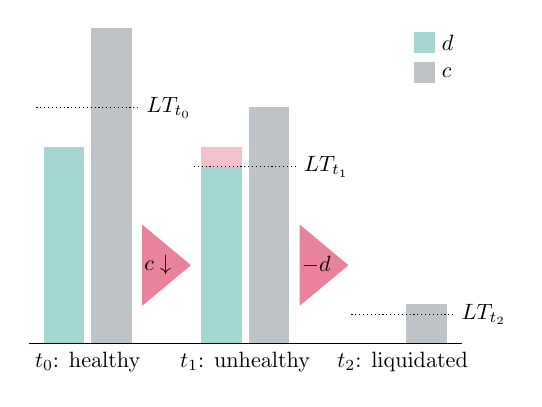
\begin{tikzpicture}[scale=0.5, every node/.style={scale=0.8}]
			
% t0

\filldraw[color = mint] (0.4,0) rectangle ++(1,5);
\filldraw[color = brightanthracite] (1.6,0) rectangle ++(1,8);

\draw [densely dotted, thin] (0.2,6) -- (2.8,6) node [right, text = black]{$LT_{t_0}$};

% t1
\uncover<2-> {
	\draw [softred, fill = softred] (2.9,3) -- (4.1,2) -- (2.9,1) -- (2.9,3) node [midway,right, text = black, xshift = -0.1cm] {$c \downarrow$} -- cycle;

	\filldraw[color = mint] (4.4,0) rectangle ++(1,5);
	\filldraw[softred!50] (4.4,4.5) rectangle ++(1,0.5);
	\filldraw[color = brightanthracite] (5.6,0) rectangle ++(1,6);

	\draw [densely dotted, thin] (4.2,4.5) -- (6.8,4.5) node [right, text = black]{$LT_{t_1}$};
}


% t2

\uncover<3->{
	\draw [softred, fill] (6.9,3) -- (8.1,2) -- (6.9,1) -- (6.9,3) node [midway,right, text = black, xshift = -0.1cm] {$-d$}  -- cycle;

	\filldraw[color = brightanthracite] (9.6,0) rectangle ++(1,1);


	\draw [densely dotted, thin] (8.2,0.75) -- (10.8,0.75) node [right, text = black]{$LT_{t_2}$};
}

% Axis with labels

\draw[-] (0,0) -- (1.5,0) node [below]{$t_0$: healthy} -- (5.5,0) node [below]{$t_1$: unhealthy} -- (9.5,0) node [below]{$t_2$: liquidated} -- (11,0);

\filldraw [mint] (9.8,7.4) rectangle ++ (0.5,0.5);
\node	at (10.3,7.65) [right] {$d$};

\filldraw [brightanthracite] (9.8,6.65) rectangle ++ (0.5,0.5);
\node	at (10.3,6.9) [right] {$c$};
		\end{tikzpicture}
		\caption{Scenario with $rLT_i = 0.75,$ $\forall i$.}
	\end{figure}
\end{minipage}
\begin{minipage}{0.38\textwidth}
	
	\uncover<2->{
	The position is open for liquidation if $aLT < \sum d_i$, i.e., if the position state is \emph{unhealthy}.
	}
	
	\vspace{1em}
	\uncover<3->{
	Collateral can now be liquidated by anyone against repayment of the 		position’s debt.
	}
\end{minipage}
	
\end{frame}
%%%	


%%%
\begin{frame}{Liquidations: Two Approaches}

Recall that protocols are unable to initiate a transaction. Instead, they have to \textbf{rely on arbitrageurs} to spot and liquidate unhealthy positions. Hence, liquidators must be incentivized. 

\uncover<2->{
\vspace{1 em}
Lending protocols use two distinct incentivization schemes.
}

\uncover<3->{
\vspace{1 em}
\textbf{1. Discount Sale} (e.g. Aave or Compound)
\vspace{0.2em}
\begin{itemize}
\item Any unhealthy position’s collateral is offered at a discount from the current on-chain oracle price.
\item Liquidator repays (part of the) position’s debt in the respective debt asset and receives collateral assets at the discounted price in return.
\end{itemize}

\vspace{0.5em}
\textbf{Pro:} Atomic transaction, fast.

\textbf{Con:} Requires high accuracy of on-chain oracle prices at all times.
}

\end{frame}
%%%	


%%%
\begin{frame}{Liquidations: Two Approaches }


\textbf{2. Collateral Auction}\\
\vspace{0.2em}
Collateral price discovery via auctions, avoiding fixed liquidator incentives. Example of a format employed by MakerDAO \cite{MakerDAO}:
\begin{itemize}
\item Dutch auction with starting price defined by oracle module. 
\item Collateral price decreases over time. 
\item Liquidators can buy any still available proportion of the collateral at current price.
\item Closes, when all debt is covered. Resets, if price falls below a certain ratio to the starting price or a duration limit is reached.
\end{itemize}
\vspace{0.5em}

\textbf{Pro:} Potentially leaving borrowers with a better collateral price.\\
\vspace{0.5em}
\textbf{Con:} Heavily depending on auction format and competition. Considerations must be given to duration, lower-bound for  prices, oracle role, and resilience during network congestions.

\end{frame}
%%%	


%%%
\begin{frame}{Flash Loans - Intuitively}

\begin{minipage}{0.3\textwidth}
	\begin{figure}
		\includegraphics[width=0.7\textwidth]{../assets/images/flashloan}	
	\end{figure}
\end{minipage}
\begin{minipage}{0.65\textwidth}
Flash Loans \textbf{do not require collateral} and can be granted in the \textbf{absence of reliable identities}. They rely on some unique properties of the EVM.
\end{minipage}

\vspace{2em}

\uncover<2-> {
\begin{minipage}{0.6\textwidth}

	Funds are borrowed, used, and repaid \textbf{within the same transaction}.

	\vspace{1em}
	Lenders rely on \textbf{transaction atomicity}: If principal plus fee cannot be paid back at the end of the transaction, all steps are reverted as if the funds were never granted.
	
\end{minipage}
\begin{minipage}{0.38\textwidth}
	\begin{figure}
		\begin{tikzpicture}[scale=0.8, every node/.style={scale=0.8}]
			
% Burger

\node at (0,0) {\includegraphics[height = 4cm]{../assets/images/burger}};

% Labels

\node at (0, 1.1) [text = darkmint] {\textbf{Borrow funds}};

\node at (0,-0.1) [text = darkmint, fill = white!50] {\textbf{Use funds at discretion}};

\node at (0,-1.3) [text = darkmint] {\textbf{Repay funds + fees}};


% Arrows

\draw [softred, fill = softred] (-0.4,0.7) -- (0.4,0.7) -- (0,0.3) -- (-0.4,0.7)  -- cycle;

\draw [softred, fill = softred] (-0.4,-0.6) -- (0.4,0-0.6) -- (0,-1) -- (-0.4,-0.6)  -- cycle;



		\end{tikzpicture}	
	\end{figure}
\end{minipage}
}
\vspace{0.5em}

\uncover<3->{
\link \href{https://eips.ethereum.org/EIPS/eip-3156}{EIP-3156: Flash Loans Specification}
}

\end{frame}
%%%	


%%%
\begin{frame}{Flash Loans - Step by Step}

\small

Let us assume that Alice wants to use a flash loan to borrow $x$ from a liquidity pool with liquidity $LP_x \geq x$. \\

\begin{enumerate}
	\item<2->[1.] Alice deploys a logic contract with an \genkey{onFlashLoan()} function that contains the code for the middle part of the sandwich. %The flash loan contract will later call the \texttt{onFlashLoan()} function of this contract. 
	\item<3->[2a.] Alice calls the \genkey{flashLoan()} function of the flash loan contract. Function arguments include the address of the logic contract, the token type and amount, as well as calldata.
	\item<4->[2b.] Flash loan contract sends $x$ to logic contract and calls \genkey{onFlashLoan()} function in Alice's logic contract, using the provided calldata.
	\item<5->[2c.] After the execution of \genkey{onFlashLoan()} has concluded, the rest of the flash loan contract's \genkey{flashLoan()} function is executed. This includes a \genkey{transferFrom()} to pull $x(1+\rho)+\bar{\rho}$, where $\rho$ is a relative fee and $\bar{\rho}$ is a flat fee. The entire transaction fails if final amount $x^* < x(1+\rho)+\bar{\rho}$ or if the logic contract did not set the necessary allowance with the flash loan contract as a spender address.
\end{enumerate}

\end{frame}
%%%	


%%%
\begin{frame}{Flash Loans - Payoff Function}

\begin{keytakeaway}{Failing Flash Loans}
		Remember: A failed transaction is still included in the blockchain but does not lead to any state changes except for the nonce update and transaction fee $\epsilon$. 
\end{keytakeaway}

\vspace{0.5 em}

\small{
\uncover<2->{
The borrower's payoff function can be expressed as:
\begin{equation*}
	\Pi = max (x^{\ast}-[x \,(1+\rho) + \bar{\rho} ],0) - \epsilon
\end{equation*}
}
}

\uncover<3->{
	\begin{figure}[t]
		\centering
		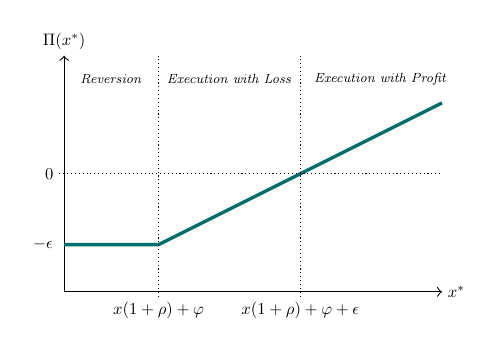
\begin{tikzpicture}[scale=0.6, every node/.style={scale=0.6}]
			
% Axis

\draw[->] (0,0) -- (0,5) node [above ]{$\Pi(x^\ast)$};
\draw[->] (0,0) -- (8,0) node [right] {$x^\ast$};


% Slope

\draw [darkmint, very thick](0,1) node [left, xshift = -0.1cm, black]{$-\epsilon$} -- (2,1) -- (8,4);


% Lines and Labels

\draw [densely dotted, thin] (-0.1,2.5)node [left, black] {$0$} -- (8,2.5);

\draw [densely dotted, thin] (2,-0.1) node [below, black]{$x(1 + \rho) + \varphi$} -- (2,5);

\draw [densely dotted, thin] (5,-0.1) node [below, black]{$x(1 + \rho) + \varphi + \epsilon$} -- (5,5);

\footnotesize

\node at (1,4.5) {\textit{Reversion}};

\node at (3.5,4.5) {\textit{Execution with Loss}};
\node at (6.7,4.5) {\textit{Execution with Profit}};
		\end{tikzpicture}
		\caption{Flash Loan Payoff Diagram \cite{FS21FlashLoans}}
	\end{figure}
}
	
\end{frame}
%%%	


%%%
\begin{frame}{Flash Loans - Applications}

Flash loans \textbf{effectively remove capital} constraints for any activity that can be performed in one blockchain transaction.

\vspace{1em}

\uncover<2->{
\textbf{Common Use Cases}:

\begin{itemize}
\item Collateral swaps
\item Arbitrage
\item Liquidations
\item Portfolio restructuring
\item ``Flash Loan Attacks'' (see key takeaway box)

\end{itemize}
}

\vspace{1em}

\uncover<3->{
\begin{keytakeaway}{Flash Loan Attacks}
	The term \textbf{Flash Loan Attack} is a misnomer. While it is true that hackers commonly use flash loans when they are attacking one or several protocols, the same attacks would also be possible without flash loans. \textbf{Flash loans only provide liquidity}. Consequently it could be argued, that flash loans have the potential to make markets more efficient and fair.
\end{keytakeaway}
}

\end{frame}
%%%	


%%%
\begin{frame}{Flash Minting}

	In some cases, protocols allow flash minting of their native token up to a certain \texttt{cap}. These tokens are \textbf{minted and burned within the same transaction}. \vspace{0.5em}
	
	\begin{itemize}
		\item<2-> This loosens the liquidity constraint $x \leq LP_x$. 
		\item<3-> Instead, the amount available to borrowers is given by:\\
			$x \leq$ \texttt{cap} $\leq$ \texttt{type(uint256).max - totalSupply()}.
	\end{itemize}
	
	\vspace{1em}
	
	\uncover<4->{
		But: Flash Minting may also introduce security challenges.
		
		\begin{itemize}
			\item e.g., if third party protocols rely on the \texttt{totalSupply} of a token as part of their security assumptions.
		\end{itemize}
	}
	
\end{frame}

%%%
\begin{frame}%[allowframebreaks]

\frametitle{References and Recommended Reading}

	\bibliographystyle{amsplain}
	\bibliography{../assets/bib/refs}
\end{frame}
%%%



\end{document}